%% \section{Compiler Correctness and Verification Techniques}

%% We review the notions of closed and open simulations
%% (\Cref{sec:overview-verification:background}), discuss the problems
%% with open simulations
%% (\Cref{sec:overview-verification:problems}) and present our solution
%% (\Cref{sec:overview-verification:solution}).
%% We also discuss the memory relations used by \ccm{} in \Cref{sec:overview-verification:injection}
%% and present mixed simulations in \Cref{sec:overview-verification:mixedsim}.


\section{\cc{}}

\subsection{Undefined Behavior}
\lipsum[1-3]

\subsection{Memory Model}
\lipsum[1-3]

\subsection{Behavioral Refinement}
\cc{}'s correctness establishes \emph{behavioral refinement}
(also called \emph{semantics preservation}) saying that
the set of all observable behaviors of a source program~$P$, denoted $\beh{P}$ (seen as a specification),
includes that of its compiled target program~$Q$, \ie $\beh{Q}$ (seen as an implementation).
Here an observable behavior of a program (either in C, assembly, or an
intermediate language) is a (finite or infinite) trace of observable events
(typically, invocation of system calls) occurring in a sequence of execution steps according to the language semantics.

The semantics of a language $\mathbb{L}$ is given by a loading
function ${\load} \in \Prgs{\mathbb{L}} \to \Memory\times\States{\mathbb{L}}$
from programs to \emph{machine states} consisting of a memory and a \emph{language state},
and a step relation
${\step} \subseteq { (\Memory\times\States{\mathbb{L}}) \times \Events \times (\Memory\times\States{\mathbb{L}})}$
between machine states producing an event.
Specifically, $\load{P}$ denotes the initial machine state after loading the program $P$, and
$(\mem,\stt) \estep{e} (\mem',\stt')$ denotes that the machine state $(\mem,\stt)$ can transition to
$(\mem',\stt')$ producing an (observable or silent) event $e$ in a single step of
execution.





\subsection{Closed Simulation}
\cc{} is a multi-pass compiler and the whole verification is performed modularly
by composing independent verification of each pass. Specifically,
verification of a pass proves that the source and target programs of every translation
performed by the pass are related by a certain relation,
called (closed) \emph{simulation}, to be described below.
Since simulation relations are closed under composition, every
end-to-end translation, which is a composition of translations of all
passes, is also related by a simulation relation. Finally, \cc{}'s
correctness follows from the fact that every simulation relation implies
behavioral refinement between the related programs.

In fact, there are two versions of simulations, \emph{forward}
and \emph{backward}.  The former is more convenient for compiler
verification but implies behavioral refinement only when the target
language is deterministic\footnote{\cc{} uses a slightly different
  condition, namely that the source language is \emph{receptive} and
  the target is \emph{determinate}.}. Since \cc{} mostly uses forward
simulations, we will also focus on forward ones throughout the paper
and discuss how to mix forward and backward simulations
to support forward reasoning even when the target language is not deterministic
in \Cref{sec:overview-verification:mixedsim}.

%% Though there are two dual notions of simulations, \emph{forward} and
%% \emph{backward}, and \cc{} mostly uses forward simulations, here we
%% focus on forward simulations for simplicity and will discuss both
%% simulations in details in \Cref{sec:overview-verification:mixedsim}.
%% \todo{========= Turn backward into forward ===========}

We say a translation of a program $P$ into $Q$ is related by a
relation $R$ between machine states if the loaded initial states
$\load{P}$ and $\load{Q}$ are related by $R$.
Then $R$ is called a (closed forward) simulation if for any
pair of machine states $(\mssrc,\mstgt)$ related by $R$, the target state $\mstgt$ simulates one step
execution of the source state $\mssrc$ (up to silent steps, denoted $\tau$) and the resulting
states are again related by $R$ (slightly simplified for presentation purposes):
\[
\begin{array}{r@{\ \ }l}
  \forall (\mssrc, \mstgt) \in R,~ \forall e, \mssrc',~&
  \mssrc \estep{e} \mssrc' \implies {}\\[1mm]
  \exists \mstgt',~&
  \mstgt \estep{\tau}^{\raisebox{-1mm}{\scriptsize$\ast$}} \estep{e}\estep{\tau}^{\raisebox{-1mm}{\scriptsize$\ast$}} \mstgt' \land (\mssrc', \mstgt') \in R~.
\end{array}
\]
%% By repeating this simulation step, one can easily see that $\beh{P} \supseteq \beh{Q}$ holds.
%% Also, it is not hard
%% to see that such simulation relations are closed under composition.
%% \jeehoon{Should we say it's a little bit simplified version?  E.g. we're omitting stuttering here.}
















\section{\ccc{}}

\subsection{Interaction Semantics}

We give a brief overview of interaction semantics of \ccc{}, which
interactively executes modules equipped with their own independent
module semantics. Each module semantics $M$ provides
a set of module states (also called \emph{cores}) $\States{M}$ with the following operations:
\begin{itemize}
\item \texttt{init\_core}: given a function $f$ with arguments $\vec{v}$,
  %and a memory $m$,
  gives the initial module state $s \in \States{M}$
  % with updated memory $m'$
  executing the invoked function $f$ with $\vec{v}$.
\item \texttt{at\_external}: given $s \in \States{M}$,
  %and a memory $m$,
  checks if an external function $f$ is called with arguments~$\vec{v}$.
  %% and if so, gives updated memory $m'$ and state $s'$.
\item \texttt{after\_external}: given $s \in \States{M}$
  where an external function is called,
  %a memory $m$
  and a return value $r$,
  gives the module state $s'$
  %and memory $m'$
  after the function call returns $r$.
\item \texttt{halted}: given $s \in \States{M}$, checks if the module execution is halted with a return value~$r$.
\item \texttt{corestep}: given $s \in \States{M}$ and memory $m$, takes a local step producing an event $e$ and the next state~$s'$ with updated memory $m'$.
\end{itemize}

We explain how interaction semantics works using an example in
\Cref{fig:inter-sem}, where the whole machine state consists of a
memory, say $m$, and a stack of module states (called \emph{core stack}), say $[s_2; s_1]$.
Then, interaction semantics checks whether the stack-top module $s_2$
is invoking an external function using \texttt{at\_external}, and if
so, pushes the invoked module's initial state, say $s_3$, obtained by
\texttt{init\_core}. Note here that the same module $M_1$ can have
multiple module states $s_1$ and $s_3$ in the stack.  Then the
new top module $s_3$ takes a local step to $s_3'$ with updated memory
$m'$ according to its \texttt{corestep}, and if $s_3'$ is a halted
state with a return value $r$ (checked with \texttt{halted}), the top
module $s_3'$ is popped and returned to the next module $s_2$, which
is then updated to $s_2'$ given by \texttt{after\_external} with the return
value $r$.

\begin{figure}[t]
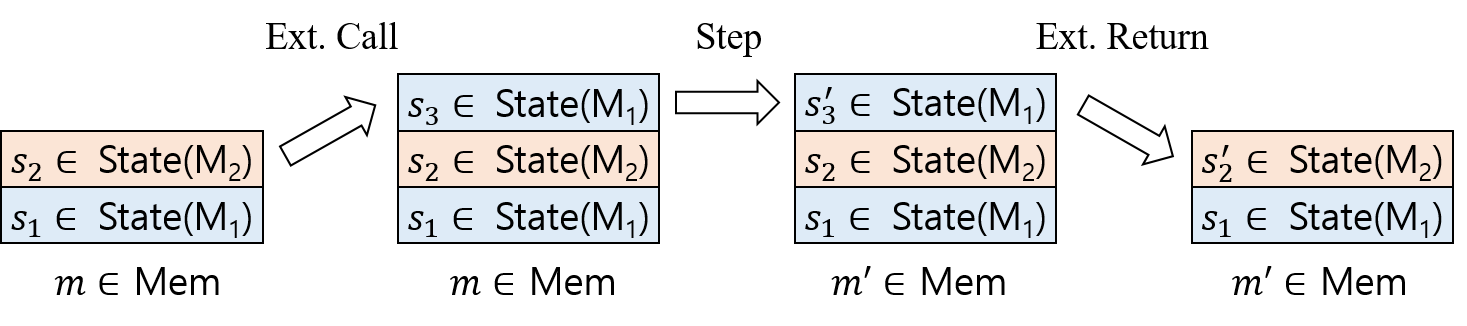
\includegraphics[width=0.9\linewidth]{images/intersem.png}
\caption{An execution of interaction semantics}
\label{fig:inter-sem}
\end{figure}

%% marshalling unmarshalling
%% marshalling the argument values into a list of values
%% setting the initial core states, unmarshalling the list of arguments.
%% at\_external: marshalling the argument values into a list of values
%% after\_external: unmarshalling the return value into
%% halted: marshalling the return value
%% corestep: use the underlying language semantics

Finally, note that the language semantics of C, assembly and
intermediate languages can be lifted to give a module semantics by
defining \texttt{corestep} to be the same as the execution step of the
language's semantics, and the other module operations to reflect the
calling conventions. Note also that all language-specific resources
(\ie other than the memory)
such as the register-file of assembly 
reside inside the module state, and thus are
duplicated at each invocation of a module.

%% One can lift a \cc{} language semantics into a core semantics by providing the interfaces:
%% Note that it is possible to define a core semantics using a mathematical specification.


\subsection{Open Simulation}
% \emph{core semantics}
The interaction semantics of \ccc{} gives a way to execute an
\emph{open} module $\module$ (\ie invoking external functions defined
outside $\module$) in isolation by providing a logical mechanism to
reflect possible interference from external function calls. More
specifically, the semantics provides two meta-level functions
$\mathtt{at\_external}$ and $\mathtt{after\_external}$. First,
$\mathtt{at\_external}~\stt = \mathtt{Some}~(f,\vec{v})$ denotes that
at language state $\stt$, an external function pointed to by a
function pointer $f$ is called with arguments $\vec{v}$. Second,
$\mathtt{after\_external}~r~\stt$ denotes the language state after the
external function call at $\stt$, assuming the call returned a value
$r$.
%% See \Cref{sec:overview-semantics:background} and \Cref{sec:main-semantics}
%% for more details about the interaction semantics.

%% $\mathtt{at\_external}$ detecting an external function call:
%% $\mathtt{at\_external}~\stt = \mathtt{Some}~(f,\vec{v})$ denotes that
%% at language state $\stt$, an external function pointed to by a
%% function pointer $f$ is called with arguments $\vec{v}$. Also, it
%% provides a meta-level function $\mathtt{after\_external}$ constructing the language state after
%% an external function call: $\mathtt{after\_external}~r~\stt$ denotes
%% the language state after the external function call at $\stt$, assuming
%% the call returned a value $r$. See \Cref{sec:main-semantics} for more details
%% about the interaction semantics.
%% \jeehoon{I don't think it's necessary to mention the word ``core semantics''. Why not just saying
%%   it's interaction semantics?}

Using interaction semantics, \ccc{} defines \emph{structured
  simulations} relating two open modules.
Here we briefly review the key ideas behind them,
which also occurred elsewhere, \eg in~\cite{pb,neis:pilsner,PLDI15}. \todo{check PLDI15}
First, unlike the closed simulations above,
structured simulations explicitly specify value and memory relations
(evolving over time) because values and memory are shared with external modules.
Specifically, such relations are defined using Kripke-style possible worlds,
called \emph{structured injections} \revision{(see \Cref{sec:overview-verification:injection} for more details)},
by giving $(i)$ a future world relation $\sqsupseteq$ for which
$w' \sqsupseteq w$ denotes that $w'$ is a future world of $w$;
and $(ii)$ value and memory relations at each world~$w$, denoted
$\mathtt{vrel}(w)$ and $\mathtt{mrel}(w)$.  Then, a
structured simulation $R$ gives a relation between machine
states at each world $w$, denoted $R(w)$, and should satisfy the
\emph{open} simulation property (simplified for presentation purposes) given in \Cref{fig:open-sim}.
\begin{figure}[t]
$
\begin{array}{@{}l@{}}
\texttt{ 1:}~\forall w,~ \forall (\memsrc,\memtgt)\in \mathtt{mrel}(w),~\forall \stsrc,\sttgt,~((\memsrc,\stsrc),(\memtgt,\sttgt))\in R(w)\implies{} \\[.5mm]
\texttt{ 2:}~\quad\textbf{match}~\mathtt{at\_external}~\stsrc~\textbf{with}\\[.5mm]
\texttt{ 3:}~\quad\mathtt{|}~\mathtt{Some}~(f_\src,\vec{v}_\src) \Rightarrow{}\\[1mm]
\texttt{ 4:}~\quad\quad \exists f_\tgt,\vec{v}_\tgt,~ \mathtt{at\_external}~\sttgt = \mathtt{Some}~(f_\tgt,\vec{v}_\tgt) \land{}\\[1mm]
\texttt{ 5:}~\quad\quad \fbox{$(f_\src,f_\tgt)\in \texttt{vrel}(w) \land (\vec{v}_\src,\vec{v}_\tgt) \in \overrightarrow{\texttt{vrel}(w)}$} \land{} \\[2mm]
\texttt{ 6:}~\quad\quad \dashbox{$\forall w' \sqsupseteq w,~\forall (\memsrc',\memtgt')\in\texttt{mrel}(w')$,}~ \dashbox{$\forall (r_\src,r_\tgt)\in \texttt{vrel}(w'),$}\\[2.5mm]
\texttt{ 7:}~\quad\quad ((\memsrc',\mathtt{after\_external}~r_\src~\stsrc),(\memtgt',\mathtt{after\_external}~r_\tgt~\sttgt))\in R(w') \\[.5mm]
\texttt{ 8:}~\quad\mathtt{|}~\mathtt{None} \Rightarrow{} \\[-.5mm]
\texttt{ 9:}~\quad\quad\forall e, \memsrc', \stsrc',~ (\memsrc, \stsrc) \estep{e} (\memsrc',\stsrc') \implies {}\\[.5mm]
\texttt{10:}~\quad\quad \exists \memtgt',\sttgt',~ (\memtgt,\sttgt) \estep{\tau}^{\raisebox{-1mm}{\scriptsize$\ast$}} \estep{e}\estep{\tau}^{\raisebox{-1mm}{\scriptsize$\ast$}} (\memtgt',\sttgt') \land{}\\[1mm]
\texttt{11:}~\quad\quad \fbox{$\exists w' \sqsupseteq w,~ (\memsrc',\memtgt') \in \mathrm{mrel}(w')$} \land {} \\[2.5mm]
\texttt{12:}~\quad\quad((\memsrc',\stsrc'), (\memtgt',\sttgt')) \in R(w')\\
\texttt{13:}~\quad\textbf{end}
\end{array}
$
\caption{Structured (or, open) simulations (simplified for presentation purposes)}
\label{fig:open-sim}
\end{figure}
% \jeehoon{In \texttt{at\_external} case, how about allowing the source to take silent steps?  Or
%   maybe we can remove silent steps also from the previous paragraph on CompCert's verification.}

Here the simulation involves rely-guarantee reasoning and is split
into two cases: one for interactions with external modules and the
other for internal steps (omitting two more cases for function start and end,
for presentation purposes). Specifically, given
any world $w$, related memories at $w$ and machine states related by
the simulation relation $R$ at $w$ (line~1), we check whether the
source state is invoking an external function or taking an internal
step (line~2). In the former case (line~3), the target state should
also be invoking an external function (line~4) and the invoked
functions and arguments should be related by the value relation at the
world~$w$ (line~5), which is a \fbox{guarantee condition} to the external modules.
Then we assume that the invoked external
functions proceed to a future world $w'$ yielding related memories and
related return values at $w'$ (line~6), which is a \dashbox{rely condition} from the external modules.
Under the assumption, the machine
states after the external calls should also be related by the
simulation relation $R$ at the future world $w'$ (line~7). In the
latter case (line~8), for any internal step from the source state
(line~9), there should be corresponding internal steps from the
target state (line~10).  Then the resulting memories after the steps
should be related at some future world $w'$ (line~11), which is a
\fbox{guarantee condition} to the external modules.  Finally, the
machine states after the steps should also be related by the
simulation relation $R$ at the future world $w'$ (line~12).

At high level, this simulation property specifies that internal
executions of the source and target modules should be related in
lockstep satisfying the guarantee conditions to the external modules,
assuming that the rely conditions from them hold after each external
function call.  Note that the rely and guarantee conditions on memory
(at lines 6 and 11) are matched and also those on values (at lines 5
and 6) will be matched if we include the omitted cases for function
start and end. This matching---in addition to the fact that the same
rely/guarantee conditions are used globally (\ie for verification of
every module)---is crucial for proving preservation of the simulation
property after linking modules because otherwise what one module
assumes about the other modules will not match with what the other
modules guarantee.

To use structured simulations for compiler verification, \ccc{} proves
the following three key properties, where we say a source module
$\module$ simulates a target module $\module'$ if there exists a
structured simulation that relates $\module$ and $\module'$:
\begin{itemize}
\item \textbf{(\emph{Vertical Compositionality})}
  If $\module$ simulates $\module'$, which simulates $\module''$,
  then $\module$ simulates~$\module''$.
\item \textbf{(\emph{Horizontal Compositionality})}
  If $\module_1$ and $\module_2$ simulate
     $\module'_1$ and $\module'_2$ respectively,
  then the linked source module  $\module_1 \llink \module_2$ simulates
  the linked target module $\module'_1 \llink \module'_2$.
\item \textbf{(\emph{Adequacy})}
  If $\module$ simulates $\module'$,
  then $\beh{\module} \supseteq \beh{\module'}$.
\end{itemize}






\subsection{Memory Relations of \cc{}}
\label{sec:overview-verification:injection:original}
%
\cc{}'s memory model consists of a finite set of blocks of finite size
and a pointer value (or, an address) is a pair $(b,o)$ of a block id $b$ and an offset $o$ inside it.
The memory identity imposes that the source and target memories are identical;
and the extension that the two memories contain identical block ids and
each target block extends the corresponding source block
with more space and any values in it at the end.

A memory injection injects a subset of the source blocks into target blocks
without overlap. More precisely, a (selected) whole source block is injected into a single target block
while allowing multiple source blocks to be injected into the same target block without overlap.
This injection map specifies the \emph{public} areas of the source and target memories and the correspondence between them.
In other words, the corresponding addresses by the injection map are treated as \emph{equivalent} (public) pointer values,
%% and therefore
so that at those corresponding addresses,
only equivalent%
\footnote{Technically speaking, \cc{} allow more undefined values in the source
  because it proves refinement rather than equivalence between the source and target programs.}
values (\ie equivalent non-pointer values or corresponding addresses) should be stored .
All the areas that are not on the injection map are considered as \emph{private} areas of the source and target memories.



